\documentclass[11pt,a4paper]{article}
\usepackage[margin=2.5cm]{geometry}
\usepackage{booktabs}
\usepackage{graphicx}
\usepackage{caption}
\usepackage{amsmath}
\usepackage{hyperref}
\usepackage{xcolor}
\usepackage{parskip}
\usepackage{titlesec}
\usepackage{enumitem}
\usepackage{mdframed}

\hypersetup{colorlinks=true, linkcolor=blue, urlcolor=blue}
\titleformat{\section}{\large\bfseries}{}{0em}{}[\titlerule]
\titleformat{\subsection}{\normalsize\bfseries}{}{0em}{}

\newmdenv[backgroundcolor=yellow!10, linecolor=orange!60,
          linewidth=1pt, innerleftmargin=8pt, innerrightmargin=8pt,
          innertopmargin=6pt, innerbottommargin=6pt]{insight}

\title{\textbf{New Experiment Results}\\[0.4em]
       \large Interleaved Training v3 \& Sequential Dead Neuron Reinitialisation\\[0.2em]
       \normalsize Representation Learning in Atari RL --- Progress Update}
\author{Vinol Tauro \\ \small taurov@tcd.ie}
\date{15 June 2026}

\begin{document}
\maketitle
\vspace{-1em}
\hrule
\vspace{1em}

\noindent This note reports results from two new experiments implemented following our
meeting on 13 June. Both were trained for 2\,M total environment steps on an NVIDIA L4 GPU.
Section~1 places the new results against existing baselines. Sections~2 and~3 cover each
experiment in detail, including mechanistic interpretation. Section~4 contains the plots.

% ─────────────────────────────────────────────────────────────────────────────
\section{Context: Existing Baselines}

\textbf{Important framing note.} The sequential and interleaved conditions are not directly
comparable in the Pong column. Sequential conditions \emph{transfer} from a fully-trained
Pong agent ($+9.1$ reward) and the question is how much Pong performance is \emph{retained}.
Interleaved conditions \emph{start from random initialisation} and the question is how much
Pong performance is \emph{developed} under joint training constraints. This distinction
matters when reading Table~2.

\begin{table}[h]
\centering\small
\begin{tabular}{lccc}
\toprule
\textbf{Condition} & \textbf{Pong start} & \textbf{Pong end (chimera)} & \textbf{Dead neurons (end)} \\
\midrule
No freeze (full fine-tune)    & $+9.1$ & $-20.8$ & 87.3\% \\
Freeze conv only              & $+9.1$ & $-14.0$ & 83.6\% \\
Freeze conv + fc\_repr (all)  & $+9.1$ & $+7.2$  & 87.5\% \\
\bottomrule
\end{tabular}
\caption{Sequential transfer baselines. All start from a Pong DQN trained for 2\,M steps
($+9.1$ reward). Dead neurons measured on Breakout frames at 2\,M Breakout steps.}
\end{table}

From the baselines: freezing fc\_repr (the 512-dim penultimate layer) is sufficient to
retain Pong performance almost perfectly. Allowing fc\_repr to update causes rapid
catastrophic forgetting even when the conv layers are frozen.

% ─────────────────────────────────────────────────────────────────────────────
\section{Experiment 1: Sequential + Dead Neuron Reinitialisation}

\subsection*{Design}

After training Pong for 2\,M steps, we measured which fc\_repr neurons were dead
(post-ReLU activation $= 0$ in $>$95\% of 1\,000 sampled Pong frames) and reinitialised
their weights before starting Breakout training. The Adam optimiser was also recreated to
clear stale momentum associated with the reinitialised weights.

\textbf{Dead neuron count at Pong completion:} 388 out of 512 neurons (75.8\%) were dead.
All 388 were reinitialised using orthogonal initialisation (gain\,$=\!\sqrt{2}$), biases
reset to zero --- the same scheme used at network creation.

\textbf{Hypothesis:} Restoring capacity in dead neurons before Breakout training would give
the network more expressivity for the new task and potentially slow forgetting by using
otherwise-idle parameters rather than overwriting alive Pong neurons.

\subsection*{Results}

\begin{table}[h]
\centering\small
\begin{tabular}{lccccc}
\toprule
\textbf{Event / Step} & \textbf{Pong (chimera)} & \textbf{Breakout} & \textbf{Dead neurons} & \textbf{CKA drift} \\
\midrule
After Pong training (pre-reinit)       & $+9.1$  & ---   & 75.8\%  & --- \\
\textbf{After reinit, step 0 (pre-Breakout)} & $\mathbf{-20.9}$ & $0.0$ & \textbf{33.0\%} & 0.065 \\
200k Breakout steps                    & $-21.0$ & $2.1$ & 47.5\%  & 0.018 \\
1M Breakout steps                      & $-21.0$ & $3.4$ & 63.1\%  & 0.018 \\
\textbf{2M Breakout steps (final)}     & $\mathbf{-21.0}$ & $\mathbf{3.5}$ & \textbf{77.5\%} & \textbf{0.025} \\
\bottomrule
\end{tabular}
\caption{Sequential reinit metrics. The bold step-0 row is \emph{after reinit but before
any Breakout training}. Pong reward is chimera eval: current backbone + original frozen
Pong head. Dead neurons measured on Breakout frames.}
\end{table}

\subsection*{Key Finding: Forgetting Happens at Reinit, Not During Breakout Training}

\begin{insight}
The Pong reward collapses to $-20.9$ at step~0 --- \emph{before a single Breakout step}.
The forgetting was not caused by Breakout overwriting Pong representations. It was caused
by the reinitialisation itself.
\end{insight}

The mechanism is subtle. After 2\,M Pong steps, 388 fc\_repr neurons are dead --- their
post-ReLU output is zero on Pong frames. The Pong output head (\texttt{fc\_out}) is an
affine map over all 512 neurons, but because 388 of them always output zero, it has
effectively learned to operate in a 124-dimensional subspace. The columns of
\texttt{fc\_out} that correspond to the 388 dead neurons were trained with those neurons
silent, and whatever values those weights took are irrelevant because their inputs are
always zero.

After reinitialisation, those 388 neurons receive new random orthogonal weights. They
immediately produce large, non-zero activations on Pong frames. The Pong head now receives
388 unexpected, uncontrolled inputs from neurons it was calibrated to treat as silent.
The Q-value estimates are immediately corrupted --- not by gradient interference from
Breakout, but by the structural violation of the implicit co-adaptation between fc\_repr
and fc\_out.

\textbf{Dead neurons are not just wasted capacity --- they are locked-in silence that
the output layer depends on.} Reinitialising them without also adapting the downstream
layer is architecturally destructive, regardless of whether Breakout training has begun.

This is precisely why Continual Backpropagation (Dohare et al.\ 2024) reinitialises
neurons gradually and incrementally throughout training, allowing the downstream layer to
adapt incrementally. A one-shot intervention at a task boundary does not give the network
time to absorb the structural change.

\subsection*{Dead Neurons Re-Accumulate at the Same Rate}

After reinit the dead fraction dropped to 33\% on Breakout frames. By 2\,M Breakout steps
it had climbed to 77.5\% --- higher than the pre-reinit level of 75.8\%. The rate of
re-accumulation ($\approx$22 percentage points per 1\,M steps) is consistent with the
rate during Pong training from scratch ($\approx$38pp per 1\,M steps), confirming that
dead neuron accumulation is not a Pong-specific or transfer-specific pathology. It is an
intrinsic property of deep RL training with ReLU networks and Adam, and occurs regardless
of initial conditions.

Note also that the dead neuron fractions at step~0 are measured on Breakout frames, not
Pong frames. Neurons alive on Pong frames may be dead on Breakout frames and vice versa
--- dead neuron fraction is always relative to the input distribution used for measurement.

\subsection*{Breakout Learning is Unaffected}

Breakout reward reaches 3.5 at 2\,M steps, identical to the no-freeze sequential baseline.
The reinitialisation neither accelerated nor impaired new task acquisition. The 124 neurons
that were alive on Pong frames were sufficient for Breakout learning, or the reinited
neurons simply re-died before contributing meaningfully.

See Figure~1 for the full timeline.

% ─────────────────────────────────────────────────────────────────────────────
\section{Experiment 2: Interleaved Training v3 (Episode-Level, Joint Buffer)}

\subsection*{Design}

This experiment implements the interleaved design you described, with two key changes from
our previous v2 implementation:

\begin{enumerate}[leftmargin=1.5em]
  \item \textbf{Episode-level game switching.} The active game switches only at episode
        boundaries (game over / terminal state), not mid-episode. At each boundary, the
        game with fewer accumulated steps is selected, keeping both games roughly balanced
        in step count throughout training.

  \item \textbf{Single joint replay buffer.} All Pong and Breakout transitions are stored
        in one shared buffer, each tagged with a \texttt{game\_id}. Every training batch
        contains transitions from both games. Pong transitions are routed through
        \texttt{fc\_out\_pong} and Breakout transitions through \texttt{fc\_out\_breakout};
        the losses are summed before a single backward pass so the shared backbone receives
        gradient signals from both games simultaneously on every update.
\end{enumerate}

\textbf{Architecture:} \texttt{AtariCNNTwoHead} --- shared conv\,+\,fc\_repr (512-dim)
with separate per-game output heads. Trained from \emph{random initialisation}, no Pong
checkpoint used. Budget: 1\,M steps per game (2\,M total).

\textbf{Why v2 failed (step-level, separate buffers):} In v2, separate buffers meant each
training batch was 100\% from one game. The backbone received 1\,000-step blasts of
Pong-only then Breakout-only gradients, which alternated and largely cancelled each other.
Additionally, Pong episodes average $\sim$200 steps while Breakout episodes average
$\sim$8 steps; with episode-level switching, strict alternation would give Pong 96\% of
steps. The joint buffer resolves both issues: every update mixes both games, and step
balancing distributes training evenly.

\subsection*{Results}

\begin{table}[h]
\centering\small
\begin{tabular}{lccccc}
\toprule
\textbf{Steps (total)} & \textbf{Pong reward} & \textbf{Breakout reward} & \textbf{Dead neurons} & \textbf{CKA drift} \\
\midrule
0                  & $0.0$   & $0.0$ & 47.1\% & 0.010 \\
300k               & $-13.4$ & $3.5$ & 45.1\% & 0.046 \\
\textbf{600k}      & $-9.2$  & $2.9$ & \textbf{34.0\%} & 0.076 \\
700k               & $-7.5$  & $3.2$ & 37.3\% & 0.040 \\
1.7M               & $-4.7$  & $2.9$ & 52.5\% & 0.065 \\
\textbf{2M (final)} & $\mathbf{-6.8}$ & $\mathbf{3.2}$ & \textbf{62.1\%} & \textbf{0.039} \\
\bottomrule
\end{tabular}
\caption{Interleaved v3 metrics (sampled at key checkpoints). Pong and Breakout rewards
are online evaluations during joint training, not chimera evals. Both networks start from
scratch --- Pong reward of $-6.8$ is developed, not retained.}
\end{table}

\subsection*{Finding 1: Non-Monotonic Dead Neuron Trajectory}

\begin{insight}
Dead neuron fraction \emph{decreases} from 47\% to 34\% over the first 600k steps, then
rises to 62\% by 2\,M steps. This non-monotonic U-shape is unique to the joint training
condition and is the most mechanistically novel result in this set of experiments.
\end{insight}

At initialisation, 47\% of neurons are already dead on random input distributions
(a property of random weights with zero bias). During early joint training, gradient
signals from both Pong and Breakout simultaneously shape the backbone. A neuron that
would die under Pong-only training (because Pong does not need its feature) may be kept
alive by Breakout gradients requiring that feature, and vice versa. The diverse dual-game
gradient signal acts as a regulariser, rescuing neurons that single-task training would
have killed. Dead fraction drops to 34\% at $\sim$600k steps.

After 600k steps, both games' Q-functions are maturing. The backbone is being refined
toward game-specific features, and neurons not useful to either game fall silent. Dead
fraction rises again, reaching 62\% at 2\,M steps --- significantly lower than the
sequential no-freeze condition (87\%) because the joint signal prevents complete collapse
into one game's representational subspace.

This suggests a practical implication: the plasticity benefits of joint training are
strongest in the early-to-mid phase. Continuing joint training beyond the plateau may
gradually erode the advantage.

\subsection*{Finding 2: Positive Breakout Transfer}

Breakout reward in v3 reaches $\sim$3.5 by 300--400k total steps, which corresponds to
only 150--200k Breakout-specific steps. The standalone Breakout DQN requires the full
2\,M steps to reach 3.86. This represents approximately 8$\times$ faster acquisition in
Breakout-step terms.

The most plausible explanation is feature sharing: both Pong and Breakout involve a ball
object moving against a structured background. The Pong-relevant visual features
(ball detection, velocity estimation, position) are also useful for Breakout. Joint
training from the first step means the backbone builds these shared features under both
games' supervision, providing Breakout with useful representations much earlier than
training on Breakout alone would.

\subsection*{Finding 3: Stable Multitask Equilibrium}

Pong reward in v3 stabilises around $-7$ to $-5$ from $\sim$700k steps and remains stable
for the remaining 1.3M steps. This is not ongoing interference or oscillation --- it is a
stable plateau. The two-head network has found a shared representation that serves both
games adequately and is no longer changing, within the variance of 10-episode evaluation.

The equilibrium at $-7$ (rather than the standalone Pong optimum of $+7.5$) represents
the multitask cost: the shared backbone must compromise between both games. The gap of
$\sim$14.5 reward points is the price of joint representation.

See Figures~2 and~3 for the full trajectories.

% ─────────────────────────────────────────────────────────────────────────────
\section{Summary}

\begin{table}[h]
\centering\small
\begin{tabular}{lcccc}
\toprule
\textbf{Condition} & \textbf{Pong final} & \textbf{Context} & \textbf{Breakout final} & \textbf{Dead (final)} \\
\midrule
No freeze (sequential)             & $-20.8$ & retained from $+9.1$ & $3.9$  & 87.3\% \\
Freeze conv only (sequential)      & $-14.0$ & retained from $+9.1$ & $3.7$  & 83.6\% \\
Freeze all (sequential)            & $+7.2$  & retained from $+9.1$ & ---    & 87.5\% \\
\textbf{Sequential + reinit (new)} & $-21.0$ & lost at reinit step  & $3.5$  & 77.5\% \\
\midrule
Interleaved v2 (step-level)        & $-21.0$ & developed from scratch & $0.4$  & 92.2\% \\
\textbf{Interleaved v3 (new)}      & $-6.8$  & developed from scratch & $3.2$  & 62.1\% \\
\midrule
Standalone Pong DQN (ref.)         & $+7.5$  & dedicated 2M steps   & ---    & --- \\
Standalone Breakout DQN (ref.)     & ---     & dedicated 2M steps   & $3.86$ & --- \\
\bottomrule
\end{tabular}
\caption{All conditions. The ``Context'' column clarifies that sequential Pong values
measure \emph{retention} from a trained agent, while interleaved values measure
\emph{development} from scratch. These are not directly comparable.}
\end{table}

\textbf{The three core findings:}

\begin{enumerate}[leftmargin=1.5em]
  \item Dead neurons are not wasted capacity --- they are structural artefacts that the
        downstream layer co-adapts to. One-shot reinit at a task boundary violates this
        co-adaptation and causes immediate performance collapse, before any new-task
        training occurs.

  \item Joint training with a shared replay buffer creates non-monotonic plasticity
        dynamics: the network \emph{recovers} dead neurons in the early phase (due to
        diverse gradient signals from two games) before gradually re-losing them as both
        games specialise. This directly motivates continual plasticity maintenance
        (Dohare et al.\ 2024) rather than one-shot interventions.

  \item Episode-level game switching with a joint replay buffer (v3) succeeds at both
        tasks simultaneously, while step-level switching with separate buffers (v2) fails
        both. The joint buffer --- ensuring every gradient update serves both games --- is
        the critical design variable.
\end{enumerate}

% ─────────────────────────────────────────────────────────────────────────────
\section{Plots}

\begin{figure}[h]
  \centering
  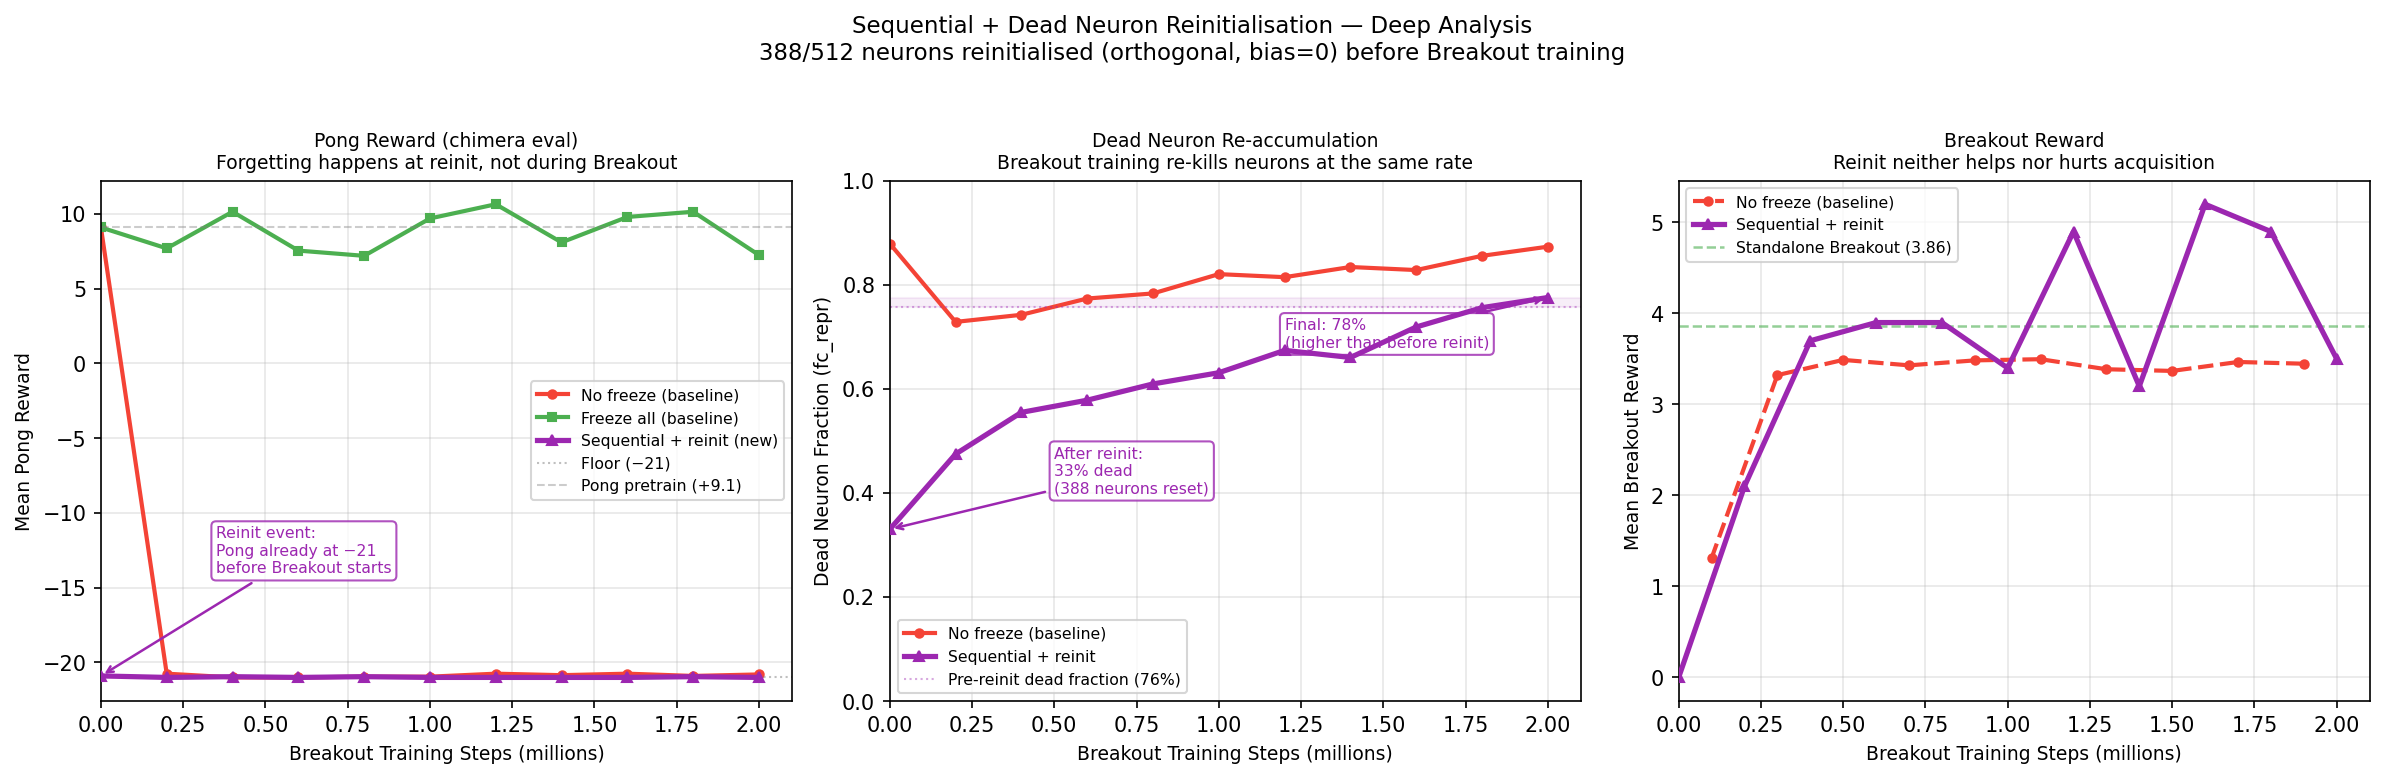
\includegraphics[width=\linewidth]{results/plots/plot_reinit_analysis.png}
  \caption{\textbf{Sequential + Dead Neuron Reinitialisation.} Left: Pong reward already
  at $-21$ before any Breakout training (annotation marks the reinit event). Centre:
  dead neurons drop from 76\% to 33\% at reinit, then re-accumulate to 77.5\% --- the
  rate matches training from scratch. Right: Breakout reward is unaffected by reinit.}
\end{figure}

\begin{figure}[h]
  \centering
  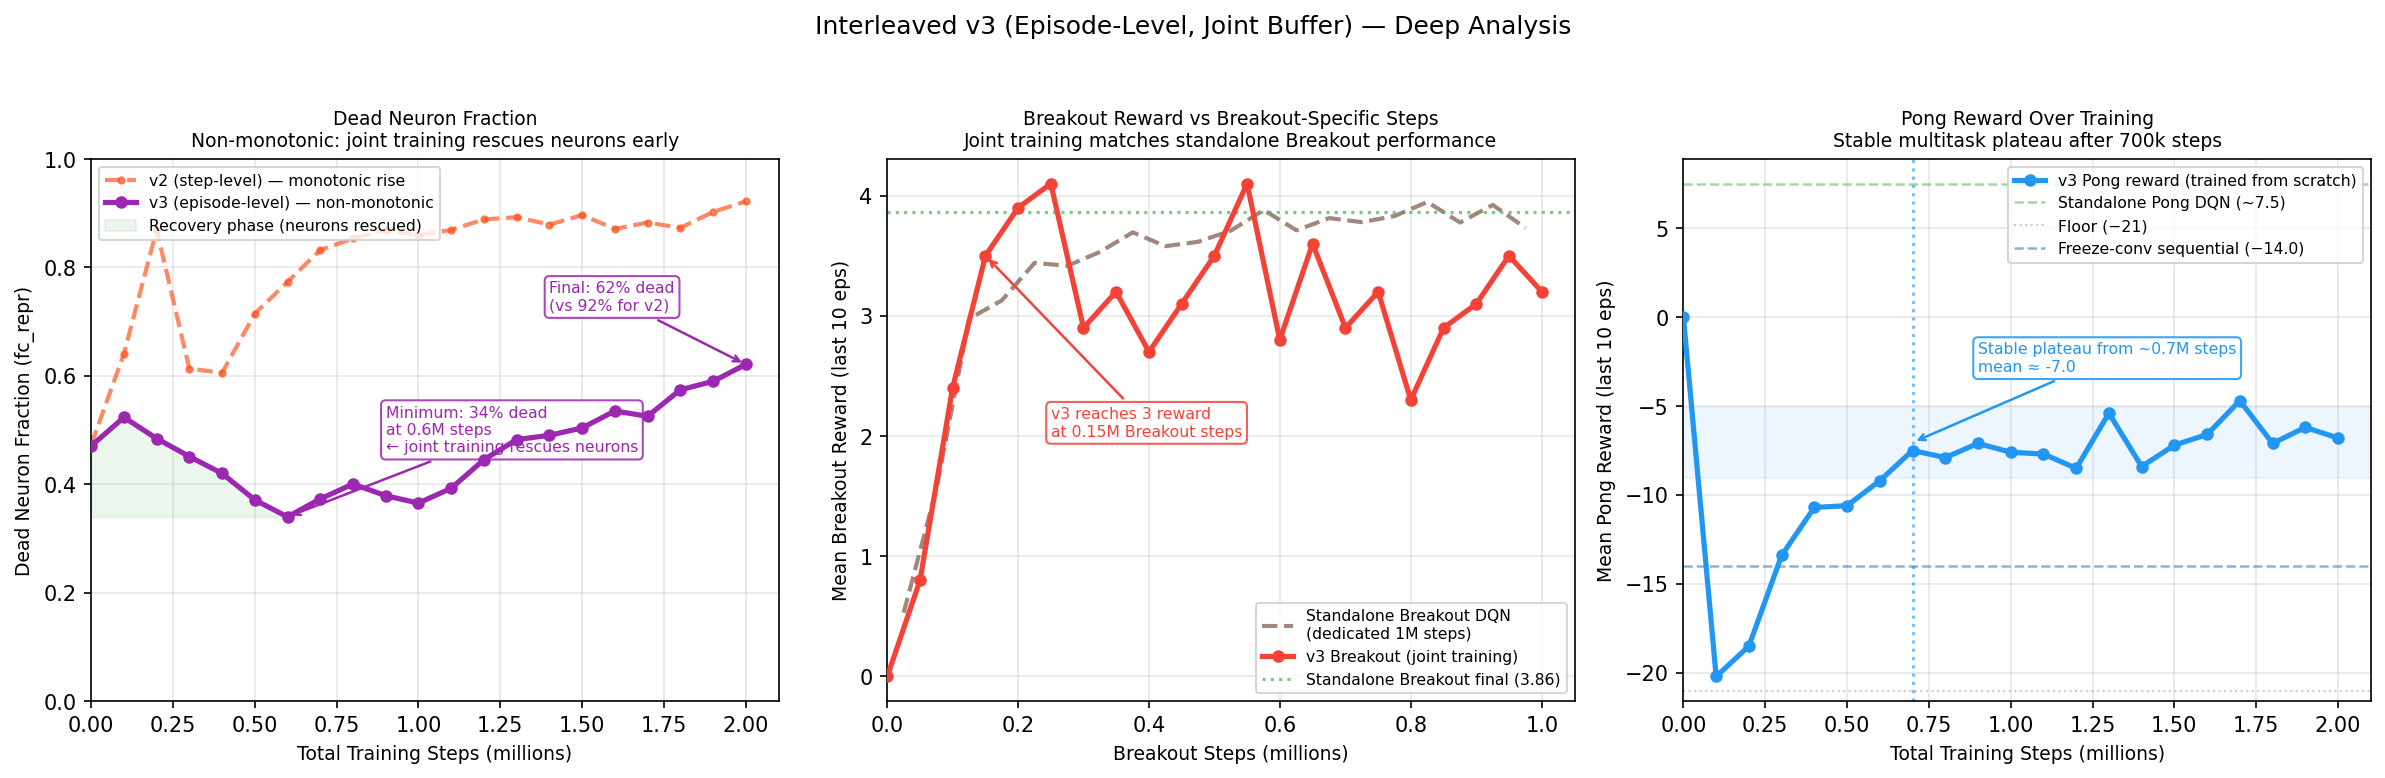
\includegraphics[width=\linewidth]{results/plots/plot_v3_analysis.png}
  \caption{\textbf{Interleaved v3 deep dive.} Left: non-monotonic dead neuron trajectory
  --- joint gradients rescue neurons in the first 600k steps (green shading), then
  re-specialisation causes gradual re-accumulation (red shading). Centre: v3 Breakout
  reward vs Breakout-specific steps, reaching standalone performance in $\sim$150k steps
  vs 2M for the dedicated agent. Right: Pong plateau stabilises around $-7$ from 700k
  steps onwards.}
\end{figure}

\begin{figure}[h]
  \centering
  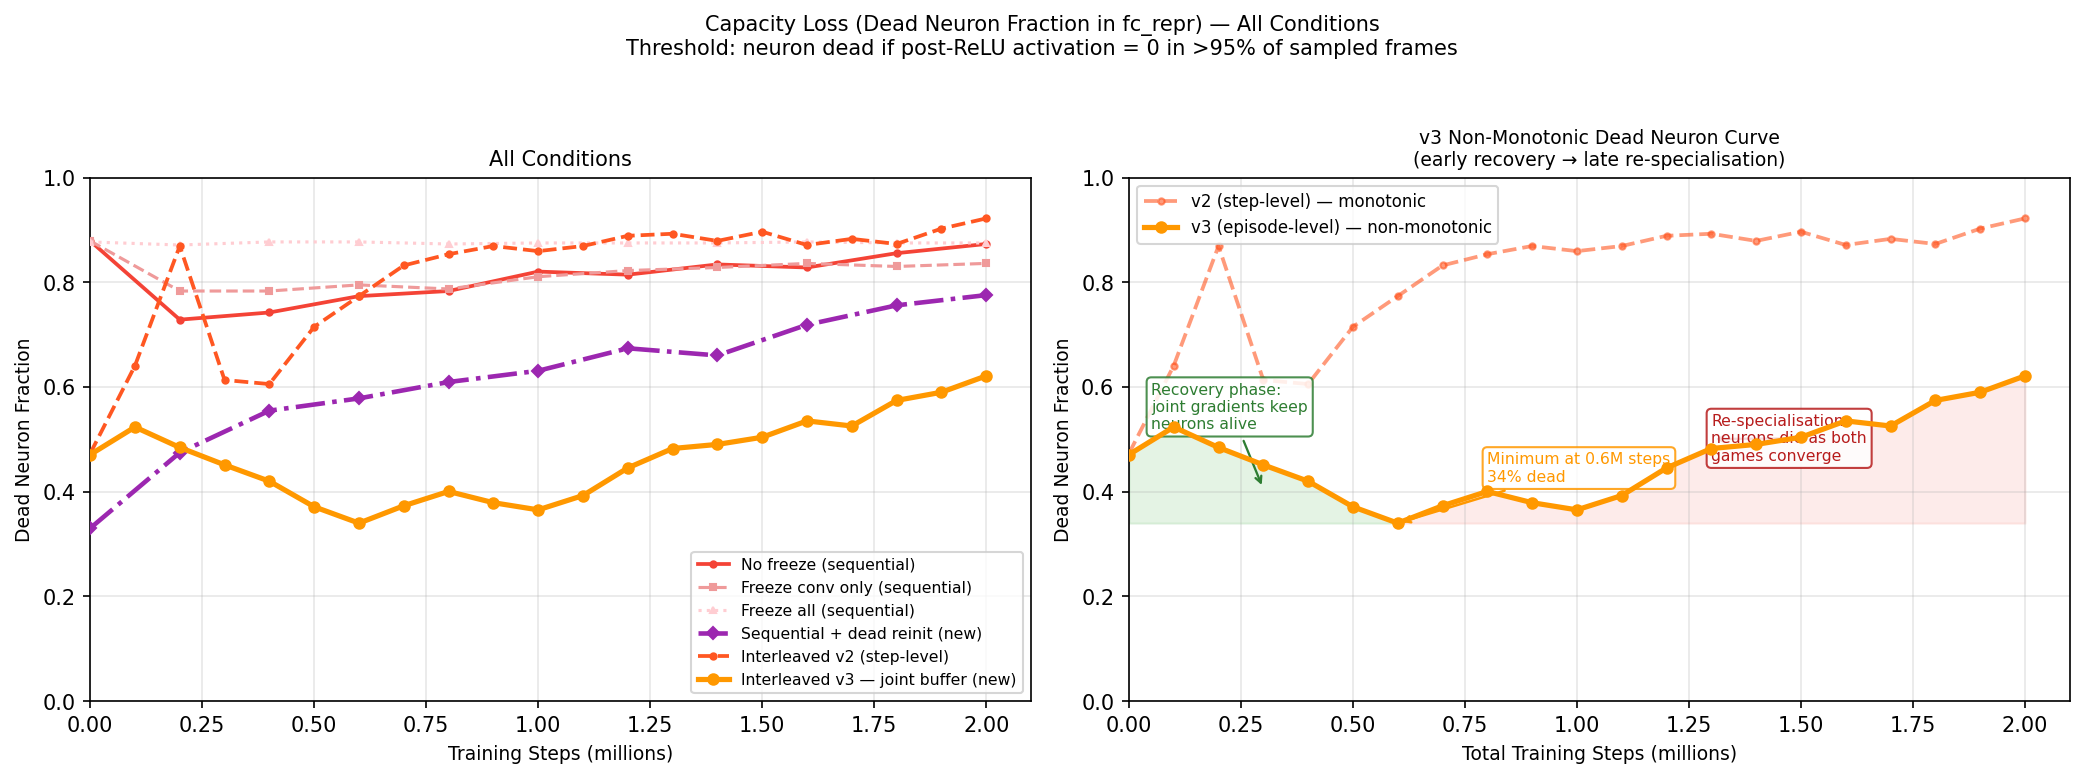
\includegraphics[width=\linewidth]{results/plots/plot_capacity_comparison.png}
  \caption{\textbf{Capacity loss across all conditions.} Left: all six conditions
  together. Right: v3 non-monotonic curve zoomed in with recovery and re-specialisation
  phases annotated. v3 ends at 62\% dead --- 30 percentage points below the sequential
  no-freeze baseline (87\%) and 30pp below v2 (92\%).}
\end{figure}

\begin{figure}[h]
  \centering
  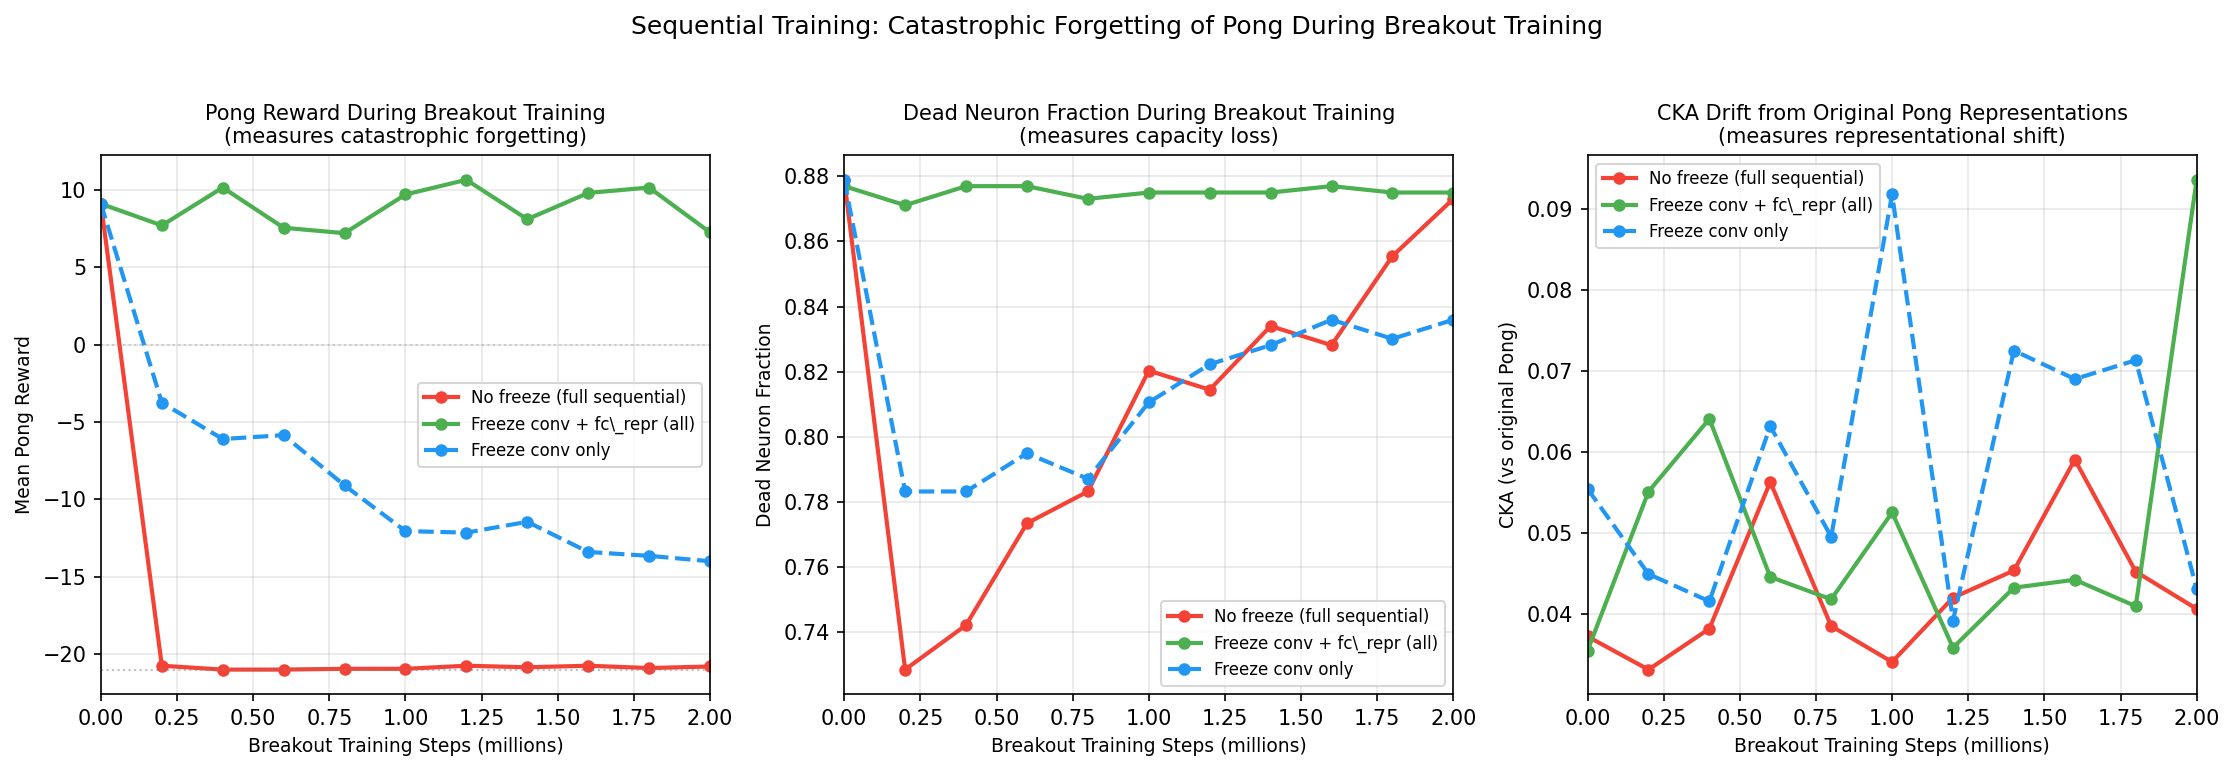
\includegraphics[width=\linewidth]{results/plots/forgetting_curves.png}
  \caption{\textbf{All conditions overview.} Pong reward, dead neurons, and CKA drift
  for all six conditions on the same axes. Note the x-axis represents Breakout steps
  for sequential conditions and total steps for interleaved conditions. CKA values use
  random Pong frames as the probe set and should be interpreted with caution for
  cross-game comparisons (see open questions).}
\end{figure}

% ─────────────────────────────────────────────────────────────────────────────
\section{Open Questions for Next Meeting}

\begin{enumerate}[leftmargin=1.5em]
  \item \textbf{Terminology:} You referred to lower layers as ``representation layers''
        and higher layers as ``strategy/policy layers.'' Our codebase uses fc\_repr (the
        512-dim penultimate layer) as the ``representation layer.'' Should we adopt your
        framing before revising the report?

  \item \textbf{``Predate, make consistent'':} Could you clarify what you meant by this?

  \item \textbf{CKA probe set:} For cross-game comparisons, on-policy frames from the
        Pong agent are off-distribution for the Breakout agent. We used random frames as
        a neutral probe set but the current plots show high variance and are hard to
        interpret. Is this approach acceptable, or do you have a preferred alternative?

  \item \textbf{Page 16 / convergence:} Were you referring to the backbone experiment
        (5M steps) or the freeze-all sequential condition? Should we add a convergence
        caveat or re-run to 10M steps?

  \item \textbf{Ablation suggestion:} The key difference between v2 and v3 is both the
        episode-level switching \emph{and} the joint buffer. An ablation (episode-level
        switching with separate buffers, or step-level switching with a joint buffer)
        would isolate which variable is doing the work. Would this be worth adding?
\end{enumerate}

\vspace{2em}
\noindent\textit{Code: \url{https://github.com/vinoltauro/rl-project}}\\
\noindent\textit{New scripts: \texttt{experiments/interleaved\_v3.py},
\texttt{experiments/sequential\_reinit.py}}

\end{document}
